\documentclass[1p]{elsarticle_modified}
%\bibliographystyle{elsarticle-num}

%\usepackage[colorlinks]{hyperref}
%\usepackage{abbrmath_seonhwa} %\Abb, \Ascr, \Acal ,\Abf, \Afrak
\usepackage{amsfonts}
\usepackage{amssymb}
\usepackage{amsmath}
\usepackage{amsthm}
\usepackage{scalefnt}
\usepackage{amsbsy}
\usepackage{kotex}
\usepackage{caption}
\usepackage{subfig}
\usepackage{color}
\usepackage{graphicx}
\usepackage{xcolor} %% white, black, red, green, blue, cyan, magenta, yellow
\usepackage{float}
\usepackage{setspace}
\usepackage{hyperref}

\usepackage{tikz}
\usetikzlibrary{arrows}

\usepackage{multirow}
\usepackage{array} % fixed length table
\usepackage{hhline}

%%%%%%%%%%%%%%%%%%%%%
\makeatletter
\renewcommand*\env@matrix[1][\arraystretch]{%
	\edef\arraystretch{#1}%
	\hskip -\arraycolsep
	\let\@ifnextchar\new@ifnextchar
	\array{*\c@MaxMatrixCols c}}
\makeatother %https://tex.stackexchange.com/questions/14071/how-can-i-increase-the-line-spacing-in-a-matrix
%%%%%%%%%%%%%%%

\usepackage[normalem]{ulem}

\newcommand{\msout}[1]{\ifmmode\text{\sout{\ensuremath{#1}}}\else\sout{#1}\fi}
%SOURCE: \msout is \stkout macro in https://tex.stackexchange.com/questions/20609/strikeout-in-math-mode

\newcommand{\cancel}[1]{
	\ifmmode
	{\color{red}\msout{#1}}
	\else
	{\color{red}\sout{#1}}
	\fi
}

\newcommand{\add}[1]{
	{\color{blue}\uwave{#1}}
}

\newcommand{\replace}[2]{
	\ifmmode
	{\color{red}\msout{#1}}{\color{blue}\uwave{#2}}
	\else
	{\color{red}\sout{#1}}{\color{blue}\uwave{#2}}
	\fi
}

\newcommand{\Sol}{\mathcal{S}} %segment
\newcommand{\D}{D} %diagram
\newcommand{\A}{\mathcal{A}} %arc


%%%%%%%%%%%%%%%%%%%%%%%%%%%%%5 test

\def\sl{\operatorname{\textup{SL}}(2,\Cbb)}
\def\psl{\operatorname{\textup{PSL}}(2,\Cbb)}
\def\quan{\mkern 1mu \triangleright \mkern 1mu}

\theoremstyle{definition}
\newtheorem{thm}{Theorem}[section]
\newtheorem{prop}[thm]{Proposition}
\newtheorem{lem}[thm]{Lemma}
\newtheorem{ques}[thm]{Question}
\newtheorem{cor}[thm]{Corollary}
\newtheorem{defn}[thm]{Definition}
\newtheorem{exam}[thm]{Example}
\newtheorem{rmk}[thm]{Remark}
\newtheorem{alg}[thm]{Algorithm}

\newcommand{\I}{\sqrt{-1}}
\begin{document}

%\begin{frontmatter}
%
%\title{Boundary parabolic representations of knots up to 8 crossings}
%
%%% Group authors per affiliation:
%\author{Yunhi Cho} 
%\address{Department of Mathematics, University of Seoul, Seoul, Korea}
%\ead{yhcho@uos.ac.kr}
%
%
%\author{Seonhwa Kim} %\fnref{s_kim}}
%\address{Center for Geometry and Physics, Institute for Basic Science, Pohang, 37673, Korea}
%\ead{ryeona17@ibs.re.kr}
%
%\author{Hyuk Kim}
%\address{Department of Mathematical Sciences, Seoul National University, Seoul 08826, Korea}
%\ead{hyukkim@snu.ac.kr}
%
%\author{Seokbeom Yoon}
%\address{Department of Mathematical Sciences, Seoul National University, Seoul, 08826,  Korea}
%\ead{sbyoon15@snu.ac.kr}
%
%\begin{abstract}
%We find all boundary parabolic representation of knots up to 8 crossings.
%
%\end{abstract}
%\begin{keyword}
%    \MSC[2010] 57M25 
%\end{keyword}
%
%\end{frontmatter}

%\linenumbers
%\tableofcontents
%
\newcommand\colored[1]{\textcolor{white}{\rule[-0.35ex]{0.8em}{1.4ex}}\kern-0.8em\color{red} #1}%
%\newcommand\colored[1]{\textcolor{white}{ #1}\kern-2.17ex	\textcolor{white}{ #1}\kern-1.81ex	\textcolor{white}{ #1}\kern-2.15ex\color{red}#1	}

{\Large $\underline{12a_{0349}~(K12a_{0349})}$}

\setlength{\tabcolsep}{10pt}
\renewcommand{\arraystretch}{1.6}
\vspace{1cm}\begin{tabular}{m{100pt}>{\centering\arraybackslash}m{274pt}}
\multirow{5}{120pt}{
	\centering
	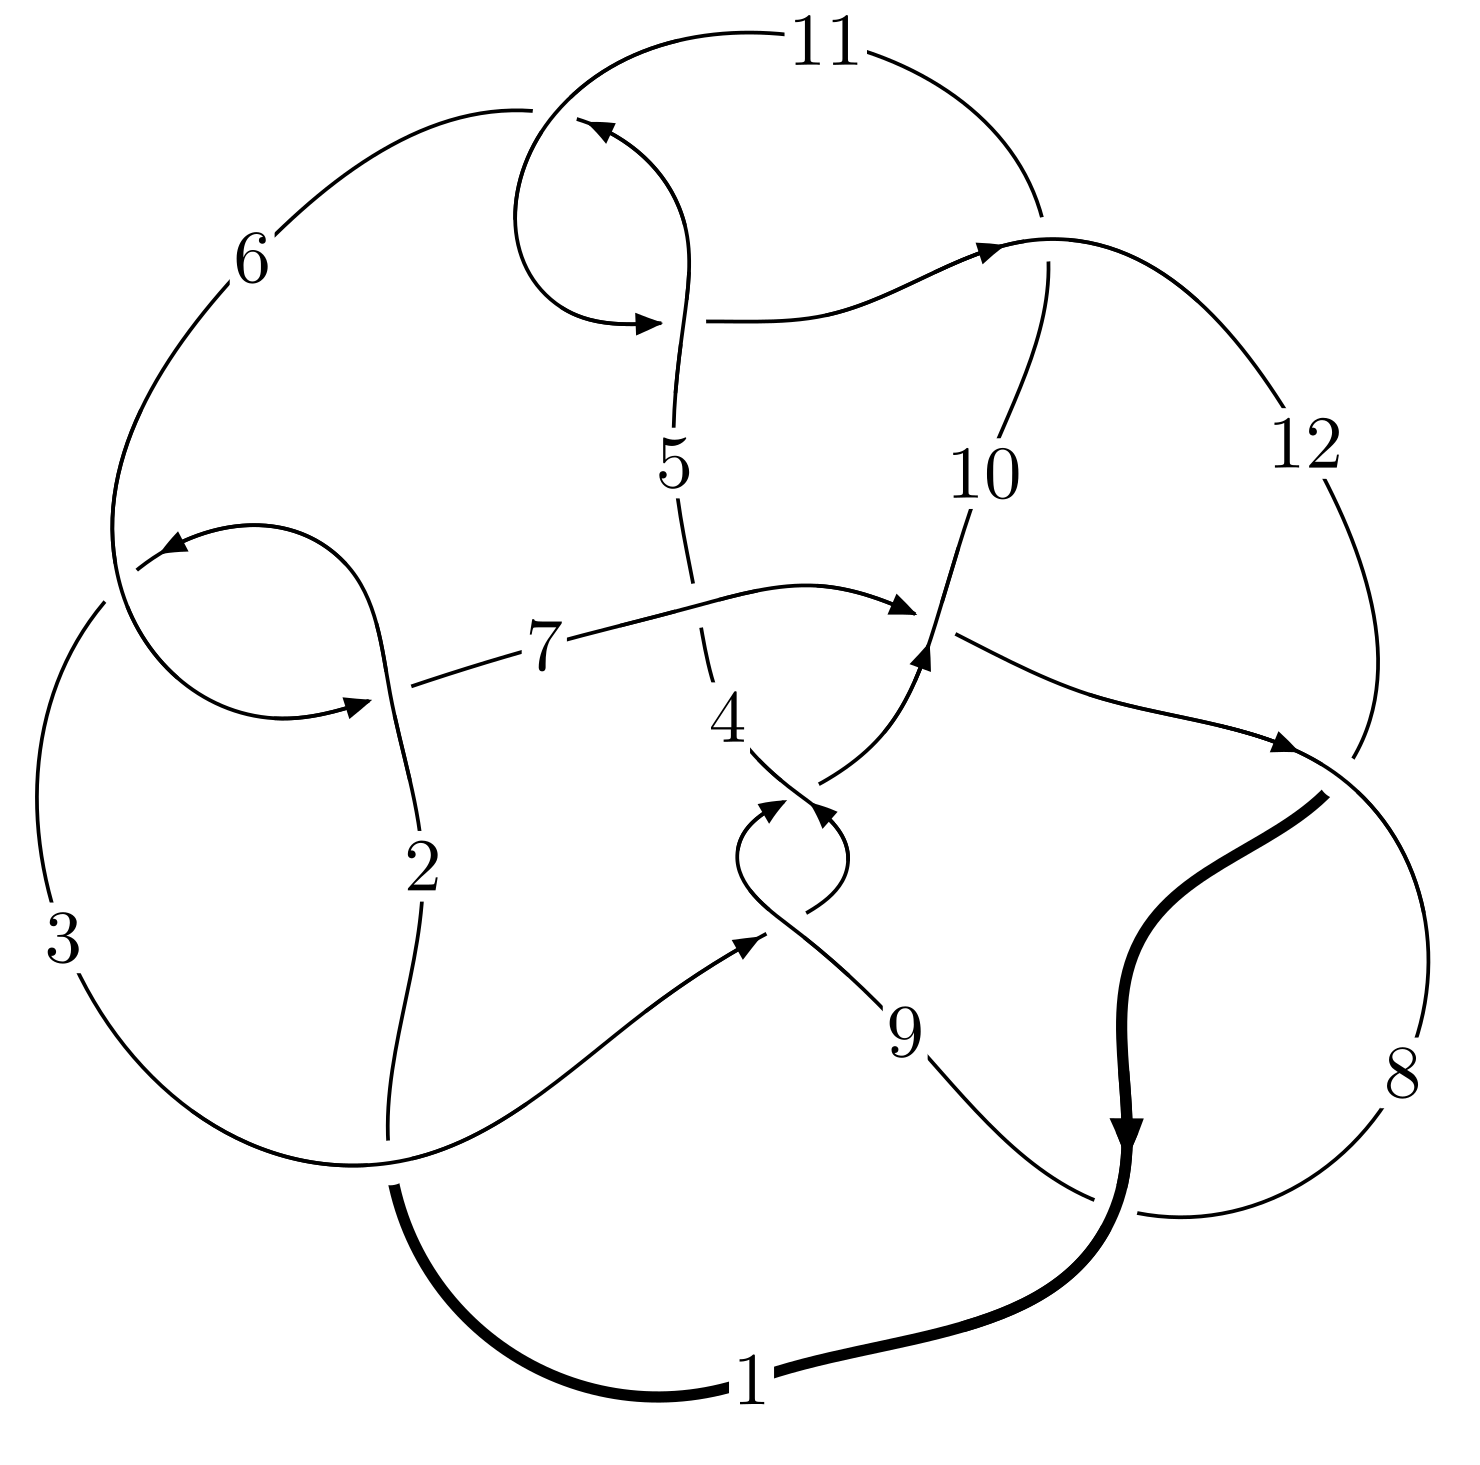
\includegraphics[width=112pt]{../../../GIT/diagram.site/Diagrams/png/1150_12a_0349.png}\\
\ \ \ A knot diagram\footnotemark}&
\allowdisplaybreaks
\textbf{Linearized knot diagam} \\
\cline{2-2}
 &
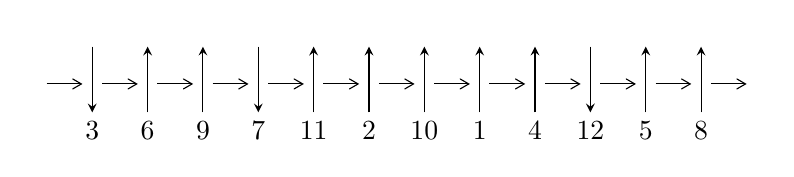
\begin{tikzpicture}[x=20pt, y=17pt]
	% nodes
	\node (C0) at (0, 0) {};
	\node (C1) at (1, 0) {};
	\node (C1U) at (1, +1) {};
	\node (C1D) at (1, -1) {3};

	\node (C2) at (2, 0) {};
	\node (C2U) at (2, +1) {};
	\node (C2D) at (2, -1) {6};

	\node (C3) at (3, 0) {};
	\node (C3U) at (3, +1) {};
	\node (C3D) at (3, -1) {9};

	\node (C4) at (4, 0) {};
	\node (C4U) at (4, +1) {};
	\node (C4D) at (4, -1) {7};

	\node (C5) at (5, 0) {};
	\node (C5U) at (5, +1) {};
	\node (C5D) at (5, -1) {11};

	\node (C6) at (6, 0) {};
	\node (C6U) at (6, +1) {};
	\node (C6D) at (6, -1) {2};

	\node (C7) at (7, 0) {};
	\node (C7U) at (7, +1) {};
	\node (C7D) at (7, -1) {10};

	\node (C8) at (8, 0) {};
	\node (C8U) at (8, +1) {};
	\node (C8D) at (8, -1) {1};

	\node (C9) at (9, 0) {};
	\node (C9U) at (9, +1) {};
	\node (C9D) at (9, -1) {4};

	\node (C10) at (10, 0) {};
	\node (C10U) at (10, +1) {};
	\node (C10D) at (10, -1) {12};

	\node (C11) at (11, 0) {};
	\node (C11U) at (11, +1) {};
	\node (C11D) at (11, -1) {5};

	\node (C12) at (12, 0) {};
	\node (C12U) at (12, +1) {};
	\node (C12D) at (12, -1) {8};
	\node (C13) at (13, 0) {};

	% arrows
	\draw[->,>={angle 60}]
	(C0) edge (C1) (C1) edge (C2) (C2) edge (C3) (C3) edge (C4) (C4) edge (C5) (C5) edge (C6) (C6) edge (C7) (C7) edge (C8) (C8) edge (C9) (C9) edge (C10) (C10) edge (C11) (C11) edge (C12) (C12) edge (C13) ;	\draw[->,>=stealth]
	(C1U) edge (C1D) (C2D) edge (C2U) (C3D) edge (C3U) (C4U) edge (C4D) (C5D) edge (C5U) (C6D) edge (C6U) (C7D) edge (C7U) (C8D) edge (C8U) (C9D) edge (C9U) (C10U) edge (C10D) (C11D) edge (C11U) (C12D) edge (C12U) ;
	\end{tikzpicture} \\
\hhline{~~} \\& 
\textbf{Solving Sequence} \\ \cline{2-2} 
 &
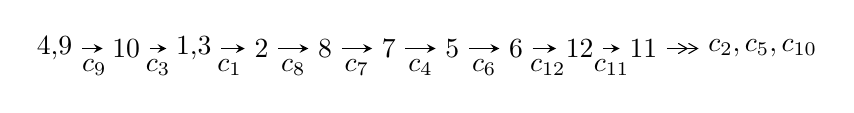
\begin{tikzpicture}[x=23pt, y=7pt]
	% node
	\node (A0) at (-1/8, 0) {4,9};
	\node (A1) at (1, 0) {10};
	\node (A2) at (33/16, 0) {1,3};
	\node (A3) at (25/8, 0) {2};
	\node (A4) at (33/8, 0) {8};
	\node (A5) at (41/8, 0) {7};
	\node (A6) at (49/8, 0) {5};
	\node (A7) at (57/8, 0) {6};
	\node (A8) at (65/8, 0) {12};
	\node (A9) at (73/8, 0) {11};
	\node (C1) at (1/2, -1) {$c_{9}$};
	\node (C2) at (3/2, -1) {$c_{3}$};
	\node (C3) at (21/8, -1) {$c_{1}$};
	\node (C4) at (29/8, -1) {$c_{8}$};
	\node (C5) at (37/8, -1) {$c_{7}$};
	\node (C6) at (45/8, -1) {$c_{4}$};
	\node (C7) at (53/8, -1) {$c_{6}$};
	\node (C8) at (61/8, -1) {$c_{12}$};
	\node (C9) at (69/8, -1) {$c_{11}$};
	\node (A10) at (11, 0) {$c_{2},c_{5},c_{10}$};

	% edge
	\draw[->,>=stealth]	
	(A0) edge (A1) (A1) edge (A2) (A2) edge (A3) (A3) edge (A4) (A4) edge (A5) (A5) edge (A6) (A6) edge (A7) (A7) edge (A8) (A8) edge (A9) ;
	\draw[->>,>={angle 60}]	
	(A9) edge (A10);
\end{tikzpicture} \\ 

\end{tabular} \\

\footnotetext{
The image of knot diagram is generated by the software ``\textbf{Draw programme}" developed by Andrew Bartholomew(\url{http://www.layer8.co.uk/maths/draw/index.htm\#Running-draw}), where we modified some parts for our purpose(\url{https://github.com/CATsTAILs/LinksPainter}).
}\phantom \\ \newline 
\centering \textbf{Ideals for irreducible components\footnotemark of $X_{\text{par}}$} 
 
\begin{align*}
I^u_{1}&=\langle 
-7.25801\times10^{614} u^{135}-1.28978\times10^{614} u^{134}+\cdots+2.94699\times10^{617} b-2.64268\times10^{619},\\
\phantom{I^u_{1}}&\phantom{= \langle  }4.49698\times10^{619} u^{135}+1.54064\times10^{619} u^{134}+\cdots+1.54007\times10^{622} a+2.15563\times10^{624},\\
\phantom{I^u_{1}}&\phantom{= \langle  }u^{136}- u^{135}+\cdots+41455 u-52259\rangle \\
I^u_{2}&=\langle 
-787618557348 u^{33}+143414944613 u^{32}+\cdots+671837590333 b-713718628306,\\
\phantom{I^u_{2}}&\phantom{= \langle  }327280736279 u^{33}-33895731689 u^{32}+\cdots+51679814641 a+286909653412,\\
\phantom{I^u_{2}}&\phantom{= \langle  }u^{34}-11 u^{32}+\cdots+2 u+1\rangle \\
\\
\end{align*}
\raggedright * 2 irreducible components of $\dim_{\mathbb{C}}=0$, with total 170 representations.\\
\footnotetext{All coefficients of polynomials are rational numbers. But the coefficients are sometimes approximated in decimal forms when there is not enough margin.}
\newpage
\renewcommand{\arraystretch}{1}
\centering \section*{I. $I^u_{1}= \langle -7.26\times10^{614} u^{135}-1.29\times10^{614} u^{134}+\cdots+2.95\times10^{617} b-2.64\times10^{619},\;4.50\times10^{619} u^{135}+1.54\times10^{619} u^{134}+\cdots+1.54\times10^{622} a+2.16\times10^{624},\;u^{136}- u^{135}+\cdots+41455 u-52259 \rangle$}
\flushleft \textbf{(i) Arc colorings}\\
\begin{tabular}{m{7pt} m{180pt} m{7pt} m{180pt} }
\flushright $a_{4}=$&$\begin{pmatrix}0\\u\end{pmatrix}$ \\
\flushright $a_{9}=$&$\begin{pmatrix}1\\0\end{pmatrix}$ \\
\flushright $a_{10}=$&$\begin{pmatrix}1\\- u^2\end{pmatrix}$ \\
\flushright $a_{1}=$&$\begin{pmatrix}-0.00291999 u^{135}-0.00100037 u^{134}+\cdots+101.594 u-139.970\\0.00246285 u^{135}+0.000437658 u^{134}+\cdots-35.2110 u+89.6737\end{pmatrix}$ \\
\flushright $a_{3}=$&$\begin{pmatrix}- u\\u\end{pmatrix}$ \\
\flushright $a_{2}=$&$\begin{pmatrix}-0.000710686 u^{135}+0.000924719 u^{134}+\cdots+83.2059 u-86.6739\\0.000253552 u^{135}-0.00148743 u^{134}+\cdots-16.8227 u+36.3776\end{pmatrix}$ \\
\flushright $a_{8}=$&$\begin{pmatrix}0.00106579 u^{135}+0.00182210 u^{134}+\cdots-77.8349 u-10.5694\\0.000388422 u^{135}-0.00145823 u^{134}+\cdots+24.4776 u+16.6686\end{pmatrix}$ \\
\flushright $a_{7}=$&$\begin{pmatrix}-0.00366961 u^{135}+0.000243350 u^{134}+\cdots-38.2923 u-178.156\\0.00811285 u^{135}+0.000328503 u^{134}+\cdots+10.1920 u+346.640\end{pmatrix}$ \\
\flushright $a_{5}=$&$\begin{pmatrix}0.00525780 u^{135}+0.00205419 u^{134}+\cdots+58.3178 u+129.963\\-0.00963619 u^{135}-0.00170547 u^{134}+\cdots+19.6587 u-336.226\end{pmatrix}$ \\
\flushright $a_{6}=$&$\begin{pmatrix}-0.00204050 u^{135}-0.000687504 u^{134}+\cdots-147.377 u-146.621\\0.00122108 u^{135}-0.000189226 u^{134}+\cdots+65.7879 u+82.7173\end{pmatrix}$ \\
\flushright $a_{12}=$&$\begin{pmatrix}0.000111542 u^{135}+0.000571574 u^{134}+\cdots+200.475 u-84.6928\\0.000506268 u^{135}+0.000750710 u^{134}+\cdots-31.0308 u+33.3645\end{pmatrix}$ \\
\flushright $a_{11}=$&$\begin{pmatrix}0.00578544 u^{135}-0.000673357 u^{134}+\cdots+34.2870 u+164.152\\-0.00420817 u^{135}+0.00119197 u^{134}+\cdots-47.0171 u-211.840\end{pmatrix}$\\&\end{tabular}
\flushleft \textbf{(ii) Obstruction class $= -1$}\\~\\
\flushleft \textbf{(iii) Cusp Shapes $= 0.0131250 u^{135}+0.00168542 u^{134}+\cdots-304.283 u+472.168$}\\~\\
\newpage\renewcommand{\arraystretch}{1}
\flushleft \textbf{(iv) u-Polynomials at the component}\newline \\
\begin{tabular}{m{50pt}|m{274pt}}
Crossings & \hspace{64pt}u-Polynomials at each crossing \\
\hline $$\begin{aligned}c_{1}\end{aligned}$$&$\begin{aligned}
&u^{136}+48 u^{135}+\cdots-102 u+1
\end{aligned}$\\
\hline $$\begin{aligned}c_{2},c_{6}\end{aligned}$$&$\begin{aligned}
&u^{136}-2 u^{135}+\cdots-16 u+1
\end{aligned}$\\
\hline $$\begin{aligned}c_{3},c_{9}\end{aligned}$$&$\begin{aligned}
&u^{136}+u^{135}+\cdots-41455 u-52259
\end{aligned}$\\
\hline $$\begin{aligned}c_{4}\end{aligned}$$&$\begin{aligned}
&u^{136}-2 u^{135}+\cdots-22083596 u+1331611
\end{aligned}$\\
\hline $$\begin{aligned}c_{5},c_{11}\end{aligned}$$&$\begin{aligned}
&u^{136}+u^{135}+\cdots-159 u-29
\end{aligned}$\\
\hline $$\begin{aligned}c_{7}\end{aligned}$$&$\begin{aligned}
&u^{136}+17 u^{135}+\cdots+2235391 u-2280599
\end{aligned}$\\
\hline $$\begin{aligned}c_{8},c_{12}\end{aligned}$$&$\begin{aligned}
&u^{136}-3 u^{135}+\cdots-39789 u-1637
\end{aligned}$\\
\hline $$\begin{aligned}c_{10}\end{aligned}$$&$\begin{aligned}
&u^{136}+57 u^{135}+\cdots+15435 u+841
\end{aligned}$\\
\hline
\end{tabular}\\~\\
\newpage\renewcommand{\arraystretch}{1}
\flushleft \textbf{(v) Riley Polynomials at the component}\newline \\
\begin{tabular}{m{50pt}|m{274pt}}
Crossings & \hspace{64pt}Riley Polynomials at each crossing \\
\hline $$\begin{aligned}c_{1}\end{aligned}$$&$\begin{aligned}
&y^{136}+96 y^{135}+\cdots-15098 y+1
\end{aligned}$\\
\hline $$\begin{aligned}c_{2},c_{6}\end{aligned}$$&$\begin{aligned}
&y^{136}+48 y^{135}+\cdots-102 y+1
\end{aligned}$\\
\hline $$\begin{aligned}c_{3},c_{9}\end{aligned}$$&$\begin{aligned}
&y^{136}-105 y^{135}+\cdots+83487901151 y+2731003081
\end{aligned}$\\
\hline $$\begin{aligned}c_{4}\end{aligned}$$&$\begin{aligned}
&y^{136}+42 y^{135}+\cdots-67453559308704 y+1773187855321
\end{aligned}$\\
\hline $$\begin{aligned}c_{5},c_{11}\end{aligned}$$&$\begin{aligned}
&y^{136}+57 y^{135}+\cdots+15435 y+841
\end{aligned}$\\
\hline $$\begin{aligned}c_{7}\end{aligned}$$&$\begin{aligned}
&y^{136}-51 y^{135}+\cdots-522376161599385 y+5201131798801
\end{aligned}$\\
\hline $$\begin{aligned}c_{8},c_{12}\end{aligned}$$&$\begin{aligned}
&y^{136}-125 y^{135}+\cdots-1327455299 y+2679769
\end{aligned}$\\
\hline $$\begin{aligned}c_{10}\end{aligned}$$&$\begin{aligned}
&y^{136}+61 y^{135}+\cdots-238478069 y+707281
\end{aligned}$\\
\hline
\end{tabular}\\~\\
\newpage\flushleft \textbf{(vi) Complex Volumes and Cusp Shapes}
$$\begin{array}{c|c|c}  
\text{Solutions to }I^u_{1}& \I (\text{vol} + \sqrt{-1}CS) & \text{Cusp shape}\\
 \hline 
\begin{aligned}
u &= -0.498799 + 0.866094 I \\
a &= -0.436060 - 0.558485 I \\
b &= \phantom{-}0.662135 - 0.538841 I\end{aligned}
 & -4.50303 - 4.74190 I & \phantom{-0.000000 } 0 \\ \hline\begin{aligned}
u &= -0.498799 - 0.866094 I \\
a &= -0.436060 + 0.558485 I \\
b &= \phantom{-}0.662135 + 0.538841 I\end{aligned}
 & -4.50303 + 4.74190 I & \phantom{-0.000000 } 0 \\ \hline\begin{aligned}
u &= \phantom{-}0.826970 + 0.600798 I \\
a &= \phantom{-}0.168212 - 0.352238 I \\
b &= \phantom{-}0.0463506 - 0.0222904 I\end{aligned}
 & -1.75800 + 2.36640 I & \phantom{-0.000000 } 0 \\ \hline\begin{aligned}
u &= \phantom{-}0.826970 - 0.600798 I \\
a &= \phantom{-}0.168212 + 0.352238 I \\
b &= \phantom{-}0.0463506 + 0.0222904 I\end{aligned}
 & -1.75800 - 2.36640 I & \phantom{-0.000000 } 0 \\ \hline\begin{aligned}
u &= \phantom{-}1.018250 + 0.368549 I \\
a &= \phantom{-}0.770491 + 0.267374 I \\
b &= \phantom{-}0.060181 - 0.841102 I\end{aligned}
 & -0.444004 + 1.297180 I & \phantom{-0.000000 } 0 \\ \hline\begin{aligned}
u &= \phantom{-}1.018250 - 0.368549 I \\
a &= \phantom{-}0.770491 - 0.267374 I \\
b &= \phantom{-}0.060181 + 0.841102 I\end{aligned}
 & -0.444004 - 1.297180 I & \phantom{-0.000000 } 0 \\ \hline\begin{aligned}
u &= \phantom{-}0.383338 + 1.045300 I \\
a &= -0.906140 - 0.397448 I \\
b &= \phantom{-}0.769089 - 0.302815 I\end{aligned}
 & -4.49772 + 1.15309 I & \phantom{-0.000000 } 0 \\ \hline\begin{aligned}
u &= \phantom{-}0.383338 - 1.045300 I \\
a &= -0.906140 + 0.397448 I \\
b &= \phantom{-}0.769089 + 0.302815 I\end{aligned}
 & -4.49772 - 1.15309 I & \phantom{-0.000000 } 0 \\ \hline\begin{aligned}
u &= \phantom{-}1.085650 + 0.250615 I \\
a &= \phantom{-}1.87655 - 0.66467 I \\
b &= -1.178100 + 0.493630 I\end{aligned}
 & \phantom{-}3.84092 - 3.61912 I & \phantom{-0.000000 } 0 \\ \hline\begin{aligned}
u &= \phantom{-}1.085650 - 0.250615 I \\
a &= \phantom{-}1.87655 + 0.66467 I \\
b &= -1.178100 - 0.493630 I\end{aligned}
 & \phantom{-}3.84092 + 3.61912 I & \phantom{-0.000000 } 0\\
 \hline 
 \end{array}$$\newpage$$\begin{array}{c|c|c}  
\text{Solutions to }I^u_{1}& \I (\text{vol} + \sqrt{-1}CS) & \text{Cusp shape}\\
 \hline 
\begin{aligned}
u &= -1.128210 + 0.248872 I \\
a &= -2.06384 - 0.62458 I \\
b &= \phantom{-}1.324680 + 0.280203 I\end{aligned}
 & \phantom{-}4.88370 - 2.14023 I & \phantom{-0.000000 } 0 \\ \hline\begin{aligned}
u &= -1.128210 - 0.248872 I \\
a &= -2.06384 + 0.62458 I \\
b &= \phantom{-}1.324680 - 0.280203 I\end{aligned}
 & \phantom{-}4.88370 + 2.14023 I & \phantom{-0.000000 } 0 \\ \hline\begin{aligned}
u &= \phantom{-}0.741762 + 0.370488 I \\
a &= -0.782095 - 0.542662 I \\
b &= \phantom{-}0.771346 + 0.548837 I\end{aligned}
 & \phantom{-}2.97325 + 6.07187 I & \phantom{-0.000000 } 0 \\ \hline\begin{aligned}
u &= \phantom{-}0.741762 - 0.370488 I \\
a &= -0.782095 + 0.542662 I \\
b &= \phantom{-}0.771346 - 0.548837 I\end{aligned}
 & \phantom{-}2.97325 - 6.07187 I & \phantom{-0.000000 } 0 \\ \hline\begin{aligned}
u &= -1.074630 + 0.468085 I \\
a &= -0.630806 + 0.475592 I \\
b &= -0.305784 - 0.924443 I\end{aligned}
 & -1.15651 - 5.70825 I & \phantom{-0.000000 } 0 \\ \hline\begin{aligned}
u &= -1.074630 - 0.468085 I \\
a &= -0.630806 - 0.475592 I \\
b &= -0.305784 + 0.924443 I\end{aligned}
 & -1.15651 + 5.70825 I & \phantom{-0.000000 } 0 \\ \hline\begin{aligned}
u &= -0.012027 + 0.819998 I \\
a &= -1.258350 - 0.607236 I \\
b &= \phantom{-}0.405550 - 0.387254 I\end{aligned}
 & -4.72424 + 1.17881 I & \phantom{-0.000000 } 0 \\ \hline\begin{aligned}
u &= -0.012027 - 0.819998 I \\
a &= -1.258350 + 0.607236 I \\
b &= \phantom{-}0.405550 + 0.387254 I\end{aligned}
 & -4.72424 - 1.17881 I & \phantom{-0.000000 } 0 \\ \hline\begin{aligned}
u &= \phantom{-}1.191520 + 0.099074 I \\
a &= \phantom{-}0.168512 - 0.219608 I \\
b &= \phantom{-}0.147167 + 1.002440 I\end{aligned}
 & -0.123641 + 0.387688 I & \phantom{-0.000000 } 0 \\ \hline\begin{aligned}
u &= \phantom{-}1.191520 - 0.099074 I \\
a &= \phantom{-}0.168512 + 0.219608 I \\
b &= \phantom{-}0.147167 - 1.002440 I\end{aligned}
 & -0.123641 - 0.387688 I & \phantom{-0.000000 } 0\\
 \hline 
 \end{array}$$\newpage$$\begin{array}{c|c|c}  
\text{Solutions to }I^u_{1}& \I (\text{vol} + \sqrt{-1}CS) & \text{Cusp shape}\\
 \hline 
\begin{aligned}
u &= -1.010380 + 0.642743 I \\
a &= -0.109222 + 0.383626 I \\
b &= -0.629395 - 0.508709 I\end{aligned}
 & -2.95195 - 0.68534 I & \phantom{-0.000000 } 0 \\ \hline\begin{aligned}
u &= -1.010380 - 0.642743 I \\
a &= -0.109222 - 0.383626 I \\
b &= -0.629395 + 0.508709 I\end{aligned}
 & -2.95195 + 0.68534 I & \phantom{-0.000000 } 0 \\ \hline\begin{aligned}
u &= -1.186750 + 0.252223 I \\
a &= -2.47939 - 0.68192 I \\
b &= \phantom{-}1.287190 - 0.242120 I\end{aligned}
 & \phantom{-}3.47467 - 4.90283 I & \phantom{-0.000000 } 0 \\ \hline\begin{aligned}
u &= -1.186750 - 0.252223 I \\
a &= -2.47939 + 0.68192 I \\
b &= \phantom{-}1.287190 + 0.242120 I\end{aligned}
 & \phantom{-}3.47467 + 4.90283 I & \phantom{-0.000000 } 0 \\ \hline\begin{aligned}
u &= \phantom{-}0.343104 + 1.167900 I \\
a &= -0.470968 + 0.106725 I \\
b &= \phantom{-}1.278080 + 0.244005 I\end{aligned}
 & \phantom{-}4.88186 + 6.91613 I & \phantom{-0.000000 } 0 \\ \hline\begin{aligned}
u &= \phantom{-}0.343104 - 1.167900 I \\
a &= -0.470968 - 0.106725 I \\
b &= \phantom{-}1.278080 - 0.244005 I\end{aligned}
 & \phantom{-}4.88186 - 6.91613 I & \phantom{-0.000000 } 0 \\ \hline\begin{aligned}
u &= \phantom{-}1.191020 + 0.251853 I \\
a &= \phantom{-}2.75012 - 0.63705 I \\
b &= -1.216870 - 0.328350 I\end{aligned}
 & \phantom{-}1.74851 + 9.99055 I & \phantom{-0.000000 } 0 \\ \hline\begin{aligned}
u &= \phantom{-}1.191020 - 0.251853 I \\
a &= \phantom{-}2.75012 + 0.63705 I \\
b &= -1.216870 + 0.328350 I\end{aligned}
 & \phantom{-}1.74851 - 9.99055 I & \phantom{-0.000000 } 0 \\ \hline\begin{aligned}
u &= -0.690025 + 0.359037 I \\
a &= \phantom{-}0.868637 - 0.357805 I \\
b &= -0.885342 + 0.367725 I\end{aligned}
 & \phantom{-}3.63008 - 0.51176 I & \phantom{-0.000000 } 0 \\ \hline\begin{aligned}
u &= -0.690025 - 0.359037 I \\
a &= \phantom{-}0.868637 + 0.357805 I \\
b &= -0.885342 - 0.367725 I\end{aligned}
 & \phantom{-}3.63008 + 0.51176 I & \phantom{-0.000000 } 0\\
 \hline 
 \end{array}$$\newpage$$\begin{array}{c|c|c}  
\text{Solutions to }I^u_{1}& \I (\text{vol} + \sqrt{-1}CS) & \text{Cusp shape}\\
 \hline 
\begin{aligned}
u &= \phantom{-}1.191760 + 0.275531 I \\
a &= \phantom{-}2.35780 - 0.27157 I \\
b &= -1.066520 - 0.108097 I\end{aligned}
 & -1.69317 + 2.87992 I & \phantom{-0.000000 } 0 \\ \hline\begin{aligned}
u &= \phantom{-}1.191760 - 0.275531 I \\
a &= \phantom{-}2.35780 + 0.27157 I \\
b &= -1.066520 + 0.108097 I\end{aligned}
 & -1.69317 - 2.87992 I & \phantom{-0.000000 } 0 \\ \hline\begin{aligned}
u &= \phantom{-}1.212320 + 0.177160 I \\
a &= -0.453222 - 0.565868 I \\
b &= \phantom{-}0.49190 + 1.36716 I\end{aligned}
 & \phantom{-}4.29649 + 6.33887 I & \phantom{-0.000000 } 0 \\ \hline\begin{aligned}
u &= \phantom{-}1.212320 - 0.177160 I \\
a &= -0.453222 + 0.565868 I \\
b &= \phantom{-}0.49190 - 1.36716 I\end{aligned}
 & \phantom{-}4.29649 - 6.33887 I & \phantom{-0.000000 } 0 \\ \hline\begin{aligned}
u &= -1.203040 + 0.251480 I \\
a &= -1.96081 - 1.03235 I \\
b &= \phantom{-}1.37829 - 0.38252 I\end{aligned}
 & \phantom{-}4.21947 - 4.92988 I & \phantom{-0.000000 } 0 \\ \hline\begin{aligned}
u &= -1.203040 - 0.251480 I \\
a &= -1.96081 + 1.03235 I \\
b &= \phantom{-}1.37829 + 0.38252 I\end{aligned}
 & \phantom{-}4.21947 + 4.92988 I & \phantom{-0.000000 } 0 \\ \hline\begin{aligned}
u &= -1.199800 + 0.276918 I \\
a &= -1.46388 - 1.80780 I \\
b &= \phantom{-}1.273200 - 0.202497 I\end{aligned}
 & \phantom{-}6.65926 - 8.40014 I & \phantom{-0.000000 } 0 \\ \hline\begin{aligned}
u &= -1.199800 - 0.276918 I \\
a &= -1.46388 + 1.80780 I \\
b &= \phantom{-}1.273200 + 0.202497 I\end{aligned}
 & \phantom{-}6.65926 + 8.40014 I & \phantom{-0.000000 } 0 \\ \hline\begin{aligned}
u &= -1.190680 + 0.337098 I \\
a &= \phantom{-}0.609368 - 0.544612 I \\
b &= -0.169824 - 0.098711 I\end{aligned}
 & \phantom{-}4.49958 + 0.42314 I & \phantom{-0.000000 } 0 \\ \hline\begin{aligned}
u &= -1.190680 - 0.337098 I \\
a &= \phantom{-}0.609368 + 0.544612 I \\
b &= -0.169824 + 0.098711 I\end{aligned}
 & \phantom{-}4.49958 - 0.42314 I & \phantom{-0.000000 } 0\\
 \hline 
 \end{array}$$\newpage$$\begin{array}{c|c|c}  
\text{Solutions to }I^u_{1}& \I (\text{vol} + \sqrt{-1}CS) & \text{Cusp shape}\\
 \hline 
\begin{aligned}
u &= \phantom{-}1.205100 + 0.283207 I \\
a &= \phantom{-}1.13403 - 1.75333 I \\
b &= -1.169630 - 0.162158 I\end{aligned}
 & \phantom{-}6.86769 + 3.46831 I & \phantom{-0.000000 } 0 \\ \hline\begin{aligned}
u &= \phantom{-}1.205100 - 0.283207 I \\
a &= \phantom{-}1.13403 + 1.75333 I \\
b &= -1.169630 + 0.162158 I\end{aligned}
 & \phantom{-}6.86769 - 3.46831 I & \phantom{-0.000000 } 0 \\ \hline\begin{aligned}
u &= \phantom{-}0.576409 + 0.493925 I \\
a &= \phantom{-}0.710298 - 0.510172 I \\
b &= -0.238780 - 0.524795 I\end{aligned}
 & -1.61585 + 1.75968 I & \phantom{-0.000000 } 0. - 5.22601 I \\ \hline\begin{aligned}
u &= \phantom{-}0.576409 - 0.493925 I \\
a &= \phantom{-}0.710298 + 0.510172 I \\
b &= -0.238780 + 0.524795 I\end{aligned}
 & -1.61585 - 1.75968 I & \phantom{-0.000000 -}0. + 5.22601 I \\ \hline\begin{aligned}
u &= -1.233510 + 0.161334 I \\
a &= \phantom{-}0.543320 - 0.322615 I \\
b &= -0.614038 + 1.201870 I\end{aligned}
 & \phantom{-}5.45984 - 0.99127 I & \phantom{-0.000000 } 0 \\ \hline\begin{aligned}
u &= -1.233510 - 0.161334 I \\
a &= \phantom{-}0.543320 + 0.322615 I \\
b &= -0.614038 - 1.201870 I\end{aligned}
 & \phantom{-}5.45984 + 0.99127 I & \phantom{-0.000000 } 0 \\ \hline\begin{aligned}
u &= -1.230320 + 0.209835 I \\
a &= -1.98825 - 0.27899 I \\
b &= \phantom{-}1.79834 - 0.75347 I\end{aligned}
 & \phantom{-}8.07893 - 2.72547 I & \phantom{-0.000000 } 0 \\ \hline\begin{aligned}
u &= -1.230320 - 0.209835 I \\
a &= -1.98825 + 0.27899 I \\
b &= \phantom{-}1.79834 + 0.75347 I\end{aligned}
 & \phantom{-}8.07893 + 2.72547 I & \phantom{-0.000000 } 0 \\ \hline\begin{aligned}
u &= \phantom{-}1.244130 + 0.214055 I \\
a &= \phantom{-}1.85177 - 0.15065 I \\
b &= -1.71200 - 0.94089 I\end{aligned}
 & \phantom{-}8.00044 + 8.02794 I & \phantom{-0.000000 } 0 \\ \hline\begin{aligned}
u &= \phantom{-}1.244130 - 0.214055 I \\
a &= \phantom{-}1.85177 + 0.15065 I \\
b &= -1.71200 + 0.94089 I\end{aligned}
 & \phantom{-}8.00044 - 8.02794 I & \phantom{-0.000000 } 0\\
 \hline 
 \end{array}$$\newpage$$\begin{array}{c|c|c}  
\text{Solutions to }I^u_{1}& \I (\text{vol} + \sqrt{-1}CS) & \text{Cusp shape}\\
 \hline 
\begin{aligned}
u &= -1.260750 + 0.101482 I \\
a &= \phantom{-}0.087206 + 0.606900 I \\
b &= -0.406888 + 0.534008 I\end{aligned}
 & \phantom{-}4.71068 + 1.16973 I & \phantom{-0.000000 } 0 \\ \hline\begin{aligned}
u &= -1.260750 - 0.101482 I \\
a &= \phantom{-}0.087206 - 0.606900 I \\
b &= -0.406888 - 0.534008 I\end{aligned}
 & \phantom{-}4.71068 - 1.16973 I & \phantom{-0.000000 } 0 \\ \hline\begin{aligned}
u &= -0.347679 + 0.646470 I \\
a &= \phantom{-}0.313440 - 0.434009 I \\
b &= -1.092720 - 0.365009 I\end{aligned}
 & \phantom{-}0.83096 + 1.63119 I & \phantom{-}6.00000 + 0. I\phantom{ +0.000000I} \\ \hline\begin{aligned}
u &= -0.347679 - 0.646470 I \\
a &= \phantom{-}0.313440 + 0.434009 I \\
b &= -1.092720 + 0.365009 I\end{aligned}
 & \phantom{-}0.83096 - 1.63119 I & \phantom{-}6.00000 + 0. I\phantom{ +0.000000I} \\ \hline\begin{aligned}
u &= \phantom{-}0.278257 + 0.678305 I \\
a &= -0.301344 - 0.828814 I \\
b &= \phantom{-}1.123340 - 0.565730 I\end{aligned}
 & -1.05120 - 6.66868 I & \phantom{-}2.28364 + 5.13023 I \\ \hline\begin{aligned}
u &= \phantom{-}0.278257 - 0.678305 I \\
a &= -0.301344 + 0.828814 I \\
b &= \phantom{-}1.123340 + 0.565730 I\end{aligned}
 & -1.05120 + 6.66868 I & \phantom{-}2.28364 - 5.13023 I \\ \hline\begin{aligned}
u &= \phantom{-}1.228330 + 0.329481 I \\
a &= -0.217156 - 0.672459 I \\
b &= -0.156344 - 0.264716 I\end{aligned}
 & \phantom{-}5.27413 + 4.87779 I & \phantom{-0.000000 } 0 \\ \hline\begin{aligned}
u &= \phantom{-}1.228330 - 0.329481 I \\
a &= -0.217156 + 0.672459 I \\
b &= -0.156344 + 0.264716 I\end{aligned}
 & \phantom{-}5.27413 - 4.87779 I & \phantom{-0.000000 } 0 \\ \hline\begin{aligned}
u &= \phantom{-}1.245780 + 0.271487 I \\
a &= \phantom{-}0.992426 - 0.577867 I \\
b &= -0.955595 - 0.707427 I\end{aligned}
 & \phantom{-}4.68025 + 5.68542 I & \phantom{-0.000000 } 0 \\ \hline\begin{aligned}
u &= \phantom{-}1.245780 - 0.271487 I \\
a &= \phantom{-}0.992426 + 0.577867 I \\
b &= -0.955595 + 0.707427 I\end{aligned}
 & \phantom{-}4.68025 - 5.68542 I & \phantom{-0.000000 } 0\\
 \hline 
 \end{array}$$\newpage$$\begin{array}{c|c|c}  
\text{Solutions to }I^u_{1}& \I (\text{vol} + \sqrt{-1}CS) & \text{Cusp shape}\\
 \hline 
\begin{aligned}
u &= -1.281220 + 0.053871 I \\
a &= \phantom{-}2.38479 + 1.15699 I \\
b &= -1.266550 - 0.012230 I\end{aligned}
 & \phantom{-}8.86520 + 4.47210 I & \phantom{-0.000000 } 0 \\ \hline\begin{aligned}
u &= -1.281220 - 0.053871 I \\
a &= \phantom{-}2.38479 - 1.15699 I \\
b &= -1.266550 + 0.012230 I\end{aligned}
 & \phantom{-}8.86520 - 4.47210 I & \phantom{-0.000000 } 0 \\ \hline\begin{aligned}
u &= \phantom{-}1.279780 + 0.092109 I \\
a &= \phantom{-}0.425482 + 0.809748 I \\
b &= \phantom{-}0.149982 + 0.361418 I\end{aligned}
 & \phantom{-}3.02656 - 6.18138 I & \phantom{-0.000000 } 0 \\ \hline\begin{aligned}
u &= \phantom{-}1.279780 - 0.092109 I \\
a &= \phantom{-}0.425482 - 0.809748 I \\
b &= \phantom{-}0.149982 - 0.361418 I\end{aligned}
 & \phantom{-}3.02656 + 6.18138 I & \phantom{-0.000000 } 0 \\ \hline\begin{aligned}
u &= \phantom{-}1.287890 + 0.038683 I \\
a &= -2.58929 + 0.80103 I \\
b &= \phantom{-}1.337830 - 0.002434 I\end{aligned}
 & \phantom{-}9.33412 + 0.55888 I & \phantom{-0.000000 } 0 \\ \hline\begin{aligned}
u &= \phantom{-}1.287890 - 0.038683 I \\
a &= -2.58929 - 0.80103 I \\
b &= \phantom{-}1.337830 + 0.002434 I\end{aligned}
 & \phantom{-}9.33412 - 0.55888 I & \phantom{-0.000000 } 0 \\ \hline\begin{aligned}
u &= -1.304960 + 0.105080 I \\
a &= \phantom{-}1.42846 + 0.60611 I \\
b &= -1.199850 + 0.396405 I\end{aligned}
 & \phantom{-}5.63228 + 0.61622 I & \phantom{-0.000000 } 0 \\ \hline\begin{aligned}
u &= -1.304960 - 0.105080 I \\
a &= \phantom{-}1.42846 - 0.60611 I \\
b &= -1.199850 - 0.396405 I\end{aligned}
 & \phantom{-}5.63228 - 0.61622 I & \phantom{-0.000000 } 0 \\ \hline\begin{aligned}
u &= -0.144459 + 1.313610 I \\
a &= -0.374310 - 0.172525 I \\
b &= \phantom{-}1.40164 - 0.33249 I\end{aligned}
 & \phantom{-}3.90971 - 12.53800 I & \phantom{-0.000000 } 0 \\ \hline\begin{aligned}
u &= -0.144459 - 1.313610 I \\
a &= -0.374310 + 0.172525 I \\
b &= \phantom{-}1.40164 + 0.33249 I\end{aligned}
 & \phantom{-}3.90971 + 12.53800 I & \phantom{-0.000000 } 0\\
 \hline 
 \end{array}$$\newpage$$\begin{array}{c|c|c}  
\text{Solutions to }I^u_{1}& \I (\text{vol} + \sqrt{-1}CS) & \text{Cusp shape}\\
 \hline 
\begin{aligned}
u &= -0.313910 + 1.287830 I \\
a &= \phantom{-}0.472119 + 0.072829 I \\
b &= -1.315130 + 0.124264 I\end{aligned}
 & \phantom{-}6.33593 - 0.51455 I & \phantom{-0.000000 } 0 \\ \hline\begin{aligned}
u &= -0.313910 - 1.287830 I \\
a &= \phantom{-}0.472119 - 0.072829 I \\
b &= -1.315130 - 0.124264 I\end{aligned}
 & \phantom{-}6.33593 + 0.51455 I & \phantom{-0.000000 } 0 \\ \hline\begin{aligned}
u &= \phantom{-}0.386398 + 0.547212 I \\
a &= -0.620616 - 0.119450 I \\
b &= \phantom{-}0.501871 + 0.419597 I\end{aligned}
 & -2.12050 + 1.59540 I & \phantom{-}3.74902 - 4.65992 I \\ \hline\begin{aligned}
u &= \phantom{-}0.386398 - 0.547212 I \\
a &= -0.620616 + 0.119450 I \\
b &= \phantom{-}0.501871 - 0.419597 I\end{aligned}
 & -2.12050 - 1.59540 I & \phantom{-}3.74902 + 4.65992 I \\ \hline\begin{aligned}
u &= \phantom{-}1.303990 + 0.281627 I \\
a &= \phantom{-}0.550886 + 0.246181 I \\
b &= -0.438250 - 1.341700 I\end{aligned}
 & \phantom{-}4.67894 + 6.58435 I & \phantom{-0.000000 } 0 \\ \hline\begin{aligned}
u &= \phantom{-}1.303990 - 0.281627 I \\
a &= \phantom{-}0.550886 - 0.246181 I \\
b &= -0.438250 + 1.341700 I\end{aligned}
 & \phantom{-}4.67894 - 6.58435 I & \phantom{-0.000000 } 0 \\ \hline\begin{aligned}
u &= -0.199724 + 0.633004 I \\
a &= -0.331527 - 0.916965 I \\
b &= \phantom{-}0.254410 - 0.849898 I\end{aligned}
 & -3.65766 + 1.54547 I & -0.60215 - 1.59690 I \\ \hline\begin{aligned}
u &= -0.199724 - 0.633004 I \\
a &= -0.331527 + 0.916965 I \\
b &= \phantom{-}0.254410 + 0.849898 I\end{aligned}
 & -3.65766 - 1.54547 I & -0.60215 + 1.59690 I \\ \hline\begin{aligned}
u &= -1.324650 + 0.279846 I \\
a &= -0.445901 + 0.495926 I \\
b &= \phantom{-}0.26082 - 1.57502 I\end{aligned}
 & \phantom{-}3.27185 - 11.77960 I & \phantom{-0.000000 } 0 \\ \hline\begin{aligned}
u &= -1.324650 - 0.279846 I \\
a &= -0.445901 - 0.495926 I \\
b &= \phantom{-}0.26082 + 1.57502 I\end{aligned}
 & \phantom{-}3.27185 + 11.77960 I & \phantom{-0.000000 } 0\\
 \hline 
 \end{array}$$\newpage$$\begin{array}{c|c|c}  
\text{Solutions to }I^u_{1}& \I (\text{vol} + \sqrt{-1}CS) & \text{Cusp shape}\\
 \hline 
\begin{aligned}
u &= -0.173911 + 0.614136 I \\
a &= -1.049210 - 0.418091 I \\
b &= -1.395700 + 0.124216 I\end{aligned}
 & \phantom{-}3.55266 + 5.08054 I & \phantom{-}7.10040 - 5.21545 I \\ \hline\begin{aligned}
u &= -0.173911 - 0.614136 I \\
a &= -1.049210 + 0.418091 I \\
b &= -1.395700 - 0.124216 I\end{aligned}
 & \phantom{-}3.55266 - 5.08054 I & \phantom{-}7.10040 + 5.21545 I \\ \hline\begin{aligned}
u &= -1.355170 + 0.164256 I \\
a &= \phantom{-}1.70136 + 0.07244 I \\
b &= -1.84388 + 0.74798 I\end{aligned}
 & \phantom{-}8.54071 - 2.54613 I & \phantom{-0.000000 } 0 \\ \hline\begin{aligned}
u &= -1.355170 - 0.164256 I \\
a &= \phantom{-}1.70136 - 0.07244 I \\
b &= -1.84388 - 0.74798 I\end{aligned}
 & \phantom{-}8.54071 + 2.54613 I & \phantom{-0.000000 } 0 \\ \hline\begin{aligned}
u &= -1.323940 + 0.336627 I \\
a &= \phantom{-}0.055473 + 0.207985 I \\
b &= -0.159194 - 1.089460 I\end{aligned}
 & -0.44519 - 5.21541 I & \phantom{-0.000000 } 0 \\ \hline\begin{aligned}
u &= -1.323940 - 0.336627 I \\
a &= \phantom{-}0.055473 - 0.207985 I \\
b &= -0.159194 + 1.089460 I\end{aligned}
 & -0.44519 + 5.21541 I & \phantom{-0.000000 } 0 \\ \hline\begin{aligned}
u &= \phantom{-}0.153358 + 0.612586 I \\
a &= \phantom{-}1.143770 - 0.331122 I \\
b &= \phantom{-}1.280970 + 0.236255 I\end{aligned}
 & \phantom{-}3.68147 - 0.12296 I & \phantom{-}7.65398 - 1.76778 I \\ \hline\begin{aligned}
u &= \phantom{-}0.153358 - 0.612586 I \\
a &= \phantom{-}1.143770 + 0.331122 I \\
b &= \phantom{-}1.280970 - 0.236255 I\end{aligned}
 & \phantom{-}3.68147 + 0.12296 I & \phantom{-}7.65398 + 1.76778 I \\ \hline\begin{aligned}
u &= \phantom{-}1.38341\phantom{ +0.000000I} \\
a &= -1.90486\phantom{ +0.000000I} \\
b &= \phantom{-}1.53700\phantom{ +0.000000I}\end{aligned}
 & \phantom{-}7.32589\phantom{ +0.000000I} & \phantom{-0.000000 } 0 \\ \hline\begin{aligned}
u &= \phantom{-}1.374800 + 0.162105 I \\
a &= -1.77587 + 0.14913 I \\
b &= \phantom{-}1.98159 + 0.57441 I\end{aligned}
 & \phantom{-}8.58778 - 2.40060 I & \phantom{-0.000000 } 0\\
 \hline 
 \end{array}$$\newpage$$\begin{array}{c|c|c}  
\text{Solutions to }I^u_{1}& \I (\text{vol} + \sqrt{-1}CS) & \text{Cusp shape}\\
 \hline 
\begin{aligned}
u &= \phantom{-}1.374800 - 0.162105 I \\
a &= -1.77587 - 0.14913 I \\
b &= \phantom{-}1.98159 - 0.57441 I\end{aligned}
 & \phantom{-}8.58778 + 2.40060 I & \phantom{-0.000000 } 0 \\ \hline\begin{aligned}
u &= -0.241389 + 0.564582 I \\
a &= -0.445724 - 0.186832 I \\
b &= -1.266660 - 0.216828 I\end{aligned}
 & \phantom{-}1.26446 + 1.87725 I & \phantom{-}1.72455 + 1.37285 I \\ \hline\begin{aligned}
u &= -0.241389 - 0.564582 I \\
a &= -0.445724 + 0.186832 I \\
b &= -1.266660 + 0.216828 I\end{aligned}
 & \phantom{-}1.26446 - 1.87725 I & \phantom{-}1.72455 - 1.37285 I \\ \hline\begin{aligned}
u &= \phantom{-}0.082523 + 1.386240 I \\
a &= \phantom{-}0.418165 - 0.123647 I \\
b &= -1.386040 - 0.226009 I\end{aligned}
 & \phantom{-}5.73615 + 6.10223 I & \phantom{-0.000000 } 0 \\ \hline\begin{aligned}
u &= \phantom{-}0.082523 - 1.386240 I \\
a &= \phantom{-}0.418165 + 0.123647 I \\
b &= -1.386040 + 0.226009 I\end{aligned}
 & \phantom{-}5.73615 - 6.10223 I & \phantom{-0.000000 } 0 \\ \hline\begin{aligned}
u &= \phantom{-}0.034917 + 0.604044 I \\
a &= -1.80374 - 0.73700 I \\
b &= -0.119066 - 0.786436 I\end{aligned}
 & -1.06796 + 8.47241 I & \phantom{-}1.49531 - 7.33951 I \\ \hline\begin{aligned}
u &= \phantom{-}0.034917 - 0.604044 I \\
a &= -1.80374 + 0.73700 I \\
b &= -0.119066 + 0.786436 I\end{aligned}
 & -1.06796 - 8.47241 I & \phantom{-}1.49531 + 7.33951 I \\ \hline\begin{aligned}
u &= \phantom{-}0.018886 + 0.595127 I \\
a &= \phantom{-}1.70036 - 0.48671 I \\
b &= \phantom{-}0.230393 - 0.537414 I\end{aligned}
 & \phantom{-}0.58538 - 3.27469 I & \phantom{-}3.78468 + 3.31399 I \\ \hline\begin{aligned}
u &= \phantom{-}0.018886 - 0.595127 I \\
a &= \phantom{-}1.70036 + 0.48671 I \\
b &= \phantom{-}0.230393 + 0.537414 I\end{aligned}
 & \phantom{-}0.58538 + 3.27469 I & \phantom{-}3.78468 - 3.31399 I \\ \hline\begin{aligned}
u &= \phantom{-}0.053723 + 0.580575 I \\
a &= -1.002380 - 0.166228 I \\
b &= -0.006400 + 0.689918 I\end{aligned}
 & \phantom{-}0.94880 - 3.60091 I & \phantom{-}5.82465 + 2.44388 I\\
 \hline 
 \end{array}$$\newpage$$\begin{array}{c|c|c}  
\text{Solutions to }I^u_{1}& \I (\text{vol} + \sqrt{-1}CS) & \text{Cusp shape}\\
 \hline 
\begin{aligned}
u &= \phantom{-}0.053723 - 0.580575 I \\
a &= -1.002380 + 0.166228 I \\
b &= -0.006400 - 0.689918 I\end{aligned}
 & \phantom{-}0.94880 + 3.60091 I & \phantom{-}5.82465 - 2.44388 I \\ \hline\begin{aligned}
u &= \phantom{-}0.020883 + 0.555314 I \\
a &= \phantom{-}1.134910 - 0.267332 I \\
b &= \phantom{-}0.197309 + 0.501629 I\end{aligned}
 & \phantom{-}1.80782 - 1.49626 I & \phantom{-}6.78415 + 3.27323 I \\ \hline\begin{aligned}
u &= \phantom{-}0.020883 - 0.555314 I \\
a &= \phantom{-}1.134910 + 0.267332 I \\
b &= \phantom{-}0.197309 - 0.501629 I\end{aligned}
 & \phantom{-}1.80782 + 1.49626 I & \phantom{-}6.78415 - 3.27323 I \\ \hline\begin{aligned}
u &= \phantom{-}1.44318 + 0.11936 I \\
a &= -1.67995 + 0.26473 I \\
b &= \phantom{-}1.82948 + 0.00577 I\end{aligned}
 & \phantom{-}6.95559 + 0.43919 I & \phantom{-0.000000 } 0 \\ \hline\begin{aligned}
u &= \phantom{-}1.44318 - 0.11936 I \\
a &= -1.67995 - 0.26473 I \\
b &= \phantom{-}1.82948 - 0.00577 I\end{aligned}
 & \phantom{-}6.95559 - 0.43919 I & \phantom{-0.000000 } 0 \\ \hline\begin{aligned}
u &= \phantom{-}0.105708 + 0.528582 I \\
a &= \phantom{-}1.354380 + 0.096403 I \\
b &= \phantom{-}0.873406 - 0.203217 I\end{aligned}
 & \phantom{-}1.16264 - 2.60619 I & \phantom{-}1.18482 + 4.75090 I \\ \hline\begin{aligned}
u &= \phantom{-}0.105708 - 0.528582 I \\
a &= \phantom{-}1.354380 - 0.096403 I \\
b &= \phantom{-}0.873406 + 0.203217 I\end{aligned}
 & \phantom{-}1.16264 + 2.60619 I & \phantom{-}1.18482 - 4.75090 I \\ \hline\begin{aligned}
u &= -0.481978\phantom{ +0.000000I} \\
a &= \phantom{-}0.594078\phantom{ +0.000000I} \\
b &= -0.416655\phantom{ +0.000000I}\end{aligned}
 & \phantom{-}0.665217\phantom{ +0.000000I} & \phantom{-}15.2060\phantom{ +0.000000I} \\ \hline\begin{aligned}
u &= -1.47784 + 0.43082 I \\
a &= \phantom{-}1.72567 + 0.47967 I \\
b &= -1.53814 + 0.45456 I\end{aligned}
 & \phantom{-}10.6735 - 12.4240 I & \phantom{-0.000000 } 0 \\ \hline\begin{aligned}
u &= -1.47784 - 0.43082 I \\
a &= \phantom{-}1.72567 - 0.47967 I \\
b &= -1.53814 - 0.45456 I\end{aligned}
 & \phantom{-}10.6735 + 12.4240 I & \phantom{-0.000000 } 0\\
 \hline 
 \end{array}$$\newpage$$\begin{array}{c|c|c}  
\text{Solutions to }I^u_{1}& \I (\text{vol} + \sqrt{-1}CS) & \text{Cusp shape}\\
 \hline 
\begin{aligned}
u &= -1.55344 + 0.10900 I \\
a &= \phantom{-}1.44157 + 0.20125 I \\
b &= -1.58035 - 0.24449 I\end{aligned}
 & \phantom{-}5.45113 + 3.49510 I & \phantom{-0.000000 } 0 \\ \hline\begin{aligned}
u &= -1.55344 - 0.10900 I \\
a &= \phantom{-}1.44157 - 0.20125 I \\
b &= -1.58035 + 0.24449 I\end{aligned}
 & \phantom{-}5.45113 - 3.49510 I & \phantom{-0.000000 } 0 \\ \hline\begin{aligned}
u &= \phantom{-}1.49935 + 0.44562 I \\
a &= -1.64231 + 0.50746 I \\
b &= \phantom{-}1.54072 + 0.38761 I\end{aligned}
 & \phantom{-}12.21970 + 6.40782 I & \phantom{-0.000000 } 0 \\ \hline\begin{aligned}
u &= \phantom{-}1.49935 - 0.44562 I \\
a &= -1.64231 - 0.50746 I \\
b &= \phantom{-}1.54072 - 0.38761 I\end{aligned}
 & \phantom{-}12.21970 - 6.40782 I & \phantom{-0.000000 } 0 \\ \hline\begin{aligned}
u &= \phantom{-}1.48354 + 0.54598 I \\
a &= \phantom{-}1.57401 - 0.62192 I \\
b &= -1.56652 - 0.56845 I\end{aligned}
 & \phantom{-}9.0849 + 18.9972 I & \phantom{-0.000000 } 0 \\ \hline\begin{aligned}
u &= \phantom{-}1.48354 - 0.54598 I \\
a &= \phantom{-}1.57401 + 0.62192 I \\
b &= -1.56652 + 0.56845 I\end{aligned}
 & \phantom{-}9.0849 - 18.9972 I & \phantom{-0.000000 } 0 \\ \hline\begin{aligned}
u &= -1.49203 + 0.56699 I \\
a &= -1.51234 - 0.64668 I \\
b &= \phantom{-}1.53994 - 0.48713 I\end{aligned}
 & \phantom{-}10.8185 - 12.8462 I & \phantom{-0.000000 } 0 \\ \hline\begin{aligned}
u &= -1.49203 - 0.56699 I \\
a &= -1.51234 + 0.64668 I \\
b &= \phantom{-}1.53994 + 0.48713 I\end{aligned}
 & \phantom{-}10.8185 + 12.8462 I & \phantom{-0.000000 } 0 \\ \hline\begin{aligned}
u &= \phantom{-}0.115668 + 0.372722 I \\
a &= \phantom{-}1.31565 + 1.61399 I \\
b &= \phantom{-}1.277090 - 0.459503 I\end{aligned}
 & \phantom{-}4.54366 - 5.65131 I & \phantom{-}8.94973 + 5.84127 I \\ \hline\begin{aligned}
u &= \phantom{-}0.115668 - 0.372722 I \\
a &= \phantom{-}1.31565 - 1.61399 I \\
b &= \phantom{-}1.277090 + 0.459503 I\end{aligned}
 & \phantom{-}4.54366 + 5.65131 I & \phantom{-}8.94973 - 5.84127 I\\
 \hline 
 \end{array}$$\newpage$$\begin{array}{c|c|c}  
\text{Solutions to }I^u_{1}& \I (\text{vol} + \sqrt{-1}CS) & \text{Cusp shape}\\
 \hline 
\begin{aligned}
u &= -0.167729 + 0.348800 I \\
a &= -0.60238 + 1.71950 I \\
b &= -1.327230 - 0.356336 I\end{aligned}
 & \phantom{-}4.83185 + 0.41381 I & \phantom{-}9.83959 + 1.29296 I \\ \hline\begin{aligned}
u &= -0.167729 - 0.348800 I \\
a &= -0.60238 - 1.71950 I \\
b &= -1.327230 + 0.356336 I\end{aligned}
 & \phantom{-}4.83185 - 0.41381 I & \phantom{-}9.83959 - 1.29296 I \\ \hline\begin{aligned}
u &= -1.58612 + 0.37026 I \\
a &= \phantom{-}1.48814 + 0.29935 I \\
b &= -1.371910 + 0.315288 I\end{aligned}
 & \phantom{-}4.88499 - 4.84019 I & \phantom{-0.000000 } 0 \\ \hline\begin{aligned}
u &= -1.58612 - 0.37026 I \\
a &= \phantom{-}1.48814 - 0.29935 I \\
b &= -1.371910 - 0.315288 I\end{aligned}
 & \phantom{-}4.88499 + 4.84019 I & \phantom{-0.000000 } 0 \\ \hline\begin{aligned}
u &= -1.52129 + 0.71461 I \\
a &= -1.226440 - 0.670369 I \\
b &= \phantom{-}1.354320 - 0.209319 I\end{aligned}
 & \phantom{-}10.12330 - 7.07095 I & \phantom{-0.000000 } 0 \\ \hline\begin{aligned}
u &= -1.52129 - 0.71461 I \\
a &= -1.226440 + 0.670369 I \\
b &= \phantom{-}1.354320 + 0.209319 I\end{aligned}
 & \phantom{-}10.12330 + 7.07095 I & \phantom{-0.000000 } 0 \\ \hline\begin{aligned}
u &= \phantom{-}1.58581 + 0.56821 I \\
a &= \phantom{-}1.38584 - 0.51723 I \\
b &= -1.312760 - 0.455900 I\end{aligned}
 & \phantom{-}3.33739 + 10.59300 I & \phantom{-0.000000 } 0 \\ \hline\begin{aligned}
u &= \phantom{-}1.58581 - 0.56821 I \\
a &= \phantom{-}1.38584 + 0.51723 I \\
b &= -1.312760 + 0.455900 I\end{aligned}
 & \phantom{-}3.33739 - 10.59300 I & \phantom{-0.000000 } 0 \\ \hline\begin{aligned}
u &= \phantom{-}1.47126 + 0.82826 I \\
a &= \phantom{-}1.075230 - 0.679854 I \\
b &= -1.265390 - 0.096333 I\end{aligned}
 & \phantom{-}7.96863 + 0.50689 I & \phantom{-0.000000 } 0 \\ \hline\begin{aligned}
u &= \phantom{-}1.47126 - 0.82826 I \\
a &= \phantom{-}1.075230 + 0.679854 I \\
b &= -1.265390 + 0.096333 I\end{aligned}
 & \phantom{-}7.96863 - 0.50689 I & \phantom{-0.000000 } 0\\
 \hline 
 \end{array}$$\newpage$$\begin{array}{c|c|c}  
\text{Solutions to }I^u_{1}& \I (\text{vol} + \sqrt{-1}CS) & \text{Cusp shape}\\
 \hline 
\begin{aligned}
u &= \phantom{-}1.62638 + 0.55149 I \\
a &= -1.283440 + 0.505916 I \\
b &= \phantom{-}1.45751 + 0.15387 I\end{aligned}
 & \phantom{-}10.86690 + 1.33856 I & \phantom{-0.000000 } 0 \\ \hline\begin{aligned}
u &= \phantom{-}1.62638 - 0.55149 I \\
a &= -1.283440 - 0.505916 I \\
b &= \phantom{-}1.45751 - 0.15387 I\end{aligned}
 & \phantom{-}10.86690 - 1.33856 I & \phantom{-0.000000 } 0 \\ \hline\begin{aligned}
u &= -1.64823 + 0.68954 I \\
a &= \phantom{-}1.101240 + 0.523659 I \\
b &= -1.413370 + 0.044625 I\end{aligned}
 & \phantom{-}8.35438 + 4.93614 I & \phantom{-0.000000 } 0 \\ \hline\begin{aligned}
u &= -1.64823 - 0.68954 I \\
a &= \phantom{-}1.101240 - 0.523659 I \\
b &= -1.413370 - 0.044625 I\end{aligned}
 & \phantom{-}8.35438 - 4.93614 I & \phantom{-0.000000 } 0 \\ \hline\begin{aligned}
u &= \phantom{-}0.13418 + 1.79441 I \\
a &= -0.586195 - 0.049213 I \\
b &= \phantom{-}1.223930 - 0.084960 I\end{aligned}
 & -2.20261 - 2.53104 I & \phantom{-0.000000 } 0 \\ \hline\begin{aligned}
u &= \phantom{-}0.13418 - 1.79441 I \\
a &= -0.586195 + 0.049213 I \\
b &= \phantom{-}1.223930 + 0.084960 I\end{aligned}
 & -2.20261 + 2.53104 I & \phantom{-0.000000 } 0\\
 \hline 
 \end{array}$$\newpage\newpage\renewcommand{\arraystretch}{1}
\centering \section*{II. $I^u_{2}= \langle -7.88\times10^{11} u^{33}+1.43\times10^{11} u^{32}+\cdots+6.72\times10^{11} b-7.14\times10^{11},\;3.27\times10^{11} u^{33}-3.39\times10^{10} u^{32}+\cdots+5.17\times10^{10} a+2.87\times10^{11},\;u^{34}-11 u^{32}+\cdots+2 u+1 \rangle$}
\flushleft \textbf{(i) Arc colorings}\\
\begin{tabular}{m{7pt} m{180pt} m{7pt} m{180pt} }
\flushright $a_{4}=$&$\begin{pmatrix}0\\u\end{pmatrix}$ \\
\flushright $a_{9}=$&$\begin{pmatrix}1\\0\end{pmatrix}$ \\
\flushright $a_{10}=$&$\begin{pmatrix}1\\- u^2\end{pmatrix}$ \\
\flushright $a_{1}=$&$\begin{pmatrix}-6.33285 u^{33}+0.655880 u^{32}+\cdots+8.20715 u-5.55168\\1.17233 u^{33}-0.213467 u^{32}+\cdots+3.51840 u+1.06234\end{pmatrix}$ \\
\flushright $a_{3}=$&$\begin{pmatrix}- u\\u\end{pmatrix}$ \\
\flushright $a_{2}=$&$\begin{pmatrix}-5.07132 u^{33}+0.451750 u^{32}+\cdots+3.93145 u-5.10926\\-0.0891988 u^{33}-0.00933745 u^{32}+\cdots+7.79409 u+0.619925\end{pmatrix}$ \\
\flushright $a_{8}=$&$\begin{pmatrix}0.729395 u^{33}-1.57109 u^{32}+\cdots+9.40657 u+9.51047\\0.0382059 u^{33}+1.04098 u^{32}+\cdots-4.41279 u-1.57109\end{pmatrix}$ \\
\flushright $a_{7}=$&$\begin{pmatrix}0.729395 u^{33}-2.57109 u^{32}+\cdots+11.4066 u+9.51047\\0.0382059 u^{33}+2.04098 u^{32}+\cdots-6.41279 u-2.57109\end{pmatrix}$ \\
\flushright $a_{5}=$&$\begin{pmatrix}5.01406 u^{33}+0.249896 u^{32}+\cdots-8.45835 u+0.740135\\1.87294 u^{33}-0.404136 u^{32}+\cdots-2.84572 u+1.90344\end{pmatrix}$ \\
\flushright $a_{6}=$&$\begin{pmatrix}1.13585 u^{33}-1.54783 u^{32}+\cdots+3.48914 u+1.78390\\0.694085 u^{33}-1.15461 u^{32}+\cdots+2.70124 u+3.76176\end{pmatrix}$ \\
\flushright $a_{12}=$&$\begin{pmatrix}-4.46974 u^{33}+1.01554 u^{32}+\cdots-1.56754 u-3.21373\\-1.14138 u^{33}-1.25053 u^{32}+\cdots+5.27064 u+0.769913\end{pmatrix}$ \\
\flushright $a_{11}=$&$\begin{pmatrix}-0.188432 u^{33}+0.711017 u^{32}+\cdots-12.8714 u-5.35223\\-1.04863 u^{33}-1.76781 u^{32}+\cdots+7.71225 u+3.02224\end{pmatrix}$\\&\end{tabular}
\flushleft \textbf{(ii) Obstruction class $= 1$}\\~\\
\flushleft \textbf{(iii) Cusp Shapes $= -\frac{2535144021258}{671837590333} u^{33}-\frac{4265588581482}{671837590333} u^{32}+\cdots+\frac{16708120824221}{671837590333} u+\frac{17275443371660}{671837590333}$}\\~\\
\newpage\renewcommand{\arraystretch}{1}
\flushleft \textbf{(iv) u-Polynomials at the component}\newline \\
\begin{tabular}{m{50pt}|m{274pt}}
Crossings & \hspace{64pt}u-Polynomials at each crossing \\
\hline $$\begin{aligned}c_{1}\end{aligned}$$&$\begin{aligned}
&u^{34}-15 u^{33}+\cdots-15 u+1
\end{aligned}$\\
\hline $$\begin{aligned}c_{2}\end{aligned}$$&$\begin{aligned}
&u^{34}- u^{33}+\cdots- u+1
\end{aligned}$\\
\hline $$\begin{aligned}c_{3}\end{aligned}$$&$\begin{aligned}
&u^{34}-11 u^{32}+\cdots-2 u+1
\end{aligned}$\\
\hline $$\begin{aligned}c_{4}\end{aligned}$$&$\begin{aligned}
&u^{34}-3 u^{33}+\cdots+5 u+1
\end{aligned}$\\
\hline $$\begin{aligned}c_{5}\end{aligned}$$&$\begin{aligned}
&u^{34}+10 u^{32}+\cdots+2 u+1
\end{aligned}$\\
\hline $$\begin{aligned}c_{6}\end{aligned}$$&$\begin{aligned}
&u^{34}+u^{33}+\cdots+u+1
\end{aligned}$\\
\hline $$\begin{aligned}c_{7}\end{aligned}$$&$\begin{aligned}
&u^{34}+4 u^{33}+\cdots+12 u+1
\end{aligned}$\\
\hline $$\begin{aligned}c_{8}\end{aligned}$$&$\begin{aligned}
&u^{34}-2 u^{33}+\cdots-14 u+1
\end{aligned}$\\
\hline $$\begin{aligned}c_{9}\end{aligned}$$&$\begin{aligned}
&u^{34}-11 u^{32}+\cdots+2 u+1
\end{aligned}$\\
\hline $$\begin{aligned}c_{10}\end{aligned}$$&$\begin{aligned}
&u^{34}-20 u^{33}+\cdots-28 u+1
\end{aligned}$\\
\hline $$\begin{aligned}c_{11}\end{aligned}$$&$\begin{aligned}
&u^{34}+10 u^{32}+\cdots-2 u+1
\end{aligned}$\\
\hline $$\begin{aligned}c_{12}\end{aligned}$$&$\begin{aligned}
&u^{34}+2 u^{33}+\cdots+14 u+1
\end{aligned}$\\
\hline
\end{tabular}\\~\\
\newpage\renewcommand{\arraystretch}{1}
\flushleft \textbf{(v) Riley Polynomials at the component}\newline \\
\begin{tabular}{m{50pt}|m{274pt}}
Crossings & \hspace{64pt}Riley Polynomials at each crossing \\
\hline $$\begin{aligned}c_{1}\end{aligned}$$&$\begin{aligned}
&y^{34}+23 y^{33}+\cdots+11 y+1
\end{aligned}$\\
\hline $$\begin{aligned}c_{2},c_{6}\end{aligned}$$&$\begin{aligned}
&y^{34}+15 y^{33}+\cdots+15 y+1
\end{aligned}$\\
\hline $$\begin{aligned}c_{3},c_{9}\end{aligned}$$&$\begin{aligned}
&y^{34}-22 y^{33}+\cdots-16 y+1
\end{aligned}$\\
\hline $$\begin{aligned}c_{4}\end{aligned}$$&$\begin{aligned}
&y^{34}+5 y^{33}+\cdots+21 y+1
\end{aligned}$\\
\hline $$\begin{aligned}c_{5},c_{11}\end{aligned}$$&$\begin{aligned}
&y^{34}+20 y^{33}+\cdots+28 y+1
\end{aligned}$\\
\hline $$\begin{aligned}c_{7}\end{aligned}$$&$\begin{aligned}
&y^{34}-8 y^{33}+\cdots-40 y+1
\end{aligned}$\\
\hline $$\begin{aligned}c_{8},c_{12}\end{aligned}$$&$\begin{aligned}
&y^{34}-38 y^{33}+\cdots-86 y+1
\end{aligned}$\\
\hline $$\begin{aligned}c_{10}\end{aligned}$$&$\begin{aligned}
&y^{34}+4 y^{33}+\cdots-64 y+1
\end{aligned}$\\
\hline
\end{tabular}\\~\\
\newpage\flushleft \textbf{(vi) Complex Volumes and Cusp Shapes}
$$\begin{array}{c|c|c}  
\text{Solutions to }I^u_{2}& \I (\text{vol} + \sqrt{-1}CS) & \text{Cusp shape}\\
 \hline 
\begin{aligned}
u &= -0.901051 + 0.514309 I \\
a &= -0.262160 + 0.279684 I \\
b &= -0.153986 - 0.606755 I\end{aligned}
 & -2.16375 - 2.02505 I & -2.39267 + 0.30437 I \\ \hline\begin{aligned}
u &= -0.901051 - 0.514309 I \\
a &= -0.262160 - 0.279684 I \\
b &= -0.153986 + 0.606755 I\end{aligned}
 & -2.16375 + 2.02505 I & -2.39267 - 0.30437 I \\ \hline\begin{aligned}
u &= \phantom{-}0.831407 + 0.470509 I \\
a &= \phantom{-}0.745619 - 0.717151 I \\
b &= \phantom{-}0.133151 + 0.051615 I\end{aligned}
 & -3.36578 + 2.02219 I & \phantom{-}0.08481 - 3.32936 I \\ \hline\begin{aligned}
u &= \phantom{-}0.831407 - 0.470509 I \\
a &= \phantom{-}0.745619 + 0.717151 I \\
b &= \phantom{-}0.133151 - 0.051615 I\end{aligned}
 & -3.36578 - 2.02219 I & \phantom{-}0.08481 + 3.32936 I \\ \hline\begin{aligned}
u &= \phantom{-}1.001050 + 0.422311 I \\
a &= \phantom{-}1.00090 - 1.02718 I \\
b &= -1.318050 - 0.305503 I\end{aligned}
 & \phantom{-}6.12005 + 1.93758 I & \phantom{-}10.72796 - 1.04035 I \\ \hline\begin{aligned}
u &= \phantom{-}1.001050 - 0.422311 I \\
a &= \phantom{-}1.00090 + 1.02718 I \\
b &= -1.318050 + 0.305503 I\end{aligned}
 & \phantom{-}6.12005 - 1.93758 I & \phantom{-}10.72796 + 1.04035 I \\ \hline\begin{aligned}
u &= \phantom{-}0.194072 + 1.094380 I \\
a &= -1.125840 - 0.513605 I \\
b &= \phantom{-}0.717799 - 0.142412 I\end{aligned}
 & -4.28029 + 1.43131 I & \phantom{-}13.6515 - 10.3289 I \\ \hline\begin{aligned}
u &= \phantom{-}0.194072 - 1.094380 I \\
a &= -1.125840 + 0.513605 I \\
b &= \phantom{-}0.717799 + 0.142412 I\end{aligned}
 & -4.28029 - 1.43131 I & \phantom{-}13.6515 + 10.3289 I \\ \hline\begin{aligned}
u &= -1.086190 + 0.298850 I \\
a &= -1.19403 - 1.11200 I \\
b &= \phantom{-}1.332450 - 0.435101 I\end{aligned}
 & \phantom{-}6.42161 - 7.11379 I & \phantom{-}11.25449 + 5.76614 I \\ \hline\begin{aligned}
u &= -1.086190 - 0.298850 I \\
a &= -1.19403 + 1.11200 I \\
b &= \phantom{-}1.332450 + 0.435101 I\end{aligned}
 & \phantom{-}6.42161 + 7.11379 I & \phantom{-}11.25449 - 5.76614 I\\
 \hline 
 \end{array}$$\newpage$$\begin{array}{c|c|c}  
\text{Solutions to }I^u_{2}& \I (\text{vol} + \sqrt{-1}CS) & \text{Cusp shape}\\
 \hline 
\begin{aligned}
u &= -0.680198 + 0.357650 I \\
a &= -1.36163 + 0.79178 I \\
b &= \phantom{-}0.719083 - 0.655685 I\end{aligned}
 & \phantom{-}2.54587 - 5.51556 I & \phantom{-}4.27046 + 2.48507 I \\ \hline\begin{aligned}
u &= -0.680198 - 0.357650 I \\
a &= -1.36163 - 0.79178 I \\
b &= \phantom{-}0.719083 + 0.655685 I\end{aligned}
 & \phantom{-}2.54587 + 5.51556 I & \phantom{-}4.27046 - 2.48507 I \\ \hline\begin{aligned}
u &= -1.223280 + 0.190245 I \\
a &= -1.54756 - 0.97220 I \\
b &= \phantom{-}1.178460 - 0.571811 I\end{aligned}
 & \phantom{-}5.15320 - 4.36862 I & \phantom{-}11.67550 + 0.90519 I \\ \hline\begin{aligned}
u &= -1.223280 - 0.190245 I \\
a &= -1.54756 + 0.97220 I \\
b &= \phantom{-}1.178460 + 0.571811 I\end{aligned}
 & \phantom{-}5.15320 + 4.36862 I & \phantom{-}11.67550 - 0.90519 I \\ \hline\begin{aligned}
u &= \phantom{-}1.299020 + 0.168024 I \\
a &= -1.82835 + 0.57508 I \\
b &= \phantom{-}1.66049 + 0.07334 I\end{aligned}
 & \phantom{-}7.83210 + 0.83769 I & \phantom{-}13.30597 - 1.15346 I \\ \hline\begin{aligned}
u &= \phantom{-}1.299020 - 0.168024 I \\
a &= -1.82835 - 0.57508 I \\
b &= \phantom{-}1.66049 - 0.07334 I\end{aligned}
 & \phantom{-}7.83210 - 0.83769 I & \phantom{-}13.30597 + 1.15346 I \\ \hline\begin{aligned}
u &= \phantom{-}0.669788 + 0.163877 I \\
a &= \phantom{-}0.71507 - 2.14236 I \\
b &= \phantom{-}0.663040 + 0.404836 I\end{aligned}
 & \phantom{-}0.46705 + 8.25996 I & \phantom{-}7.57690 - 7.27704 I \\ \hline\begin{aligned}
u &= \phantom{-}0.669788 - 0.163877 I \\
a &= \phantom{-}0.71507 + 2.14236 I \\
b &= \phantom{-}0.663040 - 0.404836 I\end{aligned}
 & \phantom{-}0.46705 - 8.25996 I & \phantom{-}7.57690 + 7.27704 I \\ \hline\begin{aligned}
u &= -1.292790 + 0.333722 I \\
a &= \phantom{-}1.42846 + 0.77075 I \\
b &= -1.51181 - 0.01223 I\end{aligned}
 & \phantom{-}6.91883 + 4.02331 I & \phantom{-}10.59648 - 4.81859 I \\ \hline\begin{aligned}
u &= -1.292790 - 0.333722 I \\
a &= \phantom{-}1.42846 - 0.77075 I \\
b &= -1.51181 + 0.01223 I\end{aligned}
 & \phantom{-}6.91883 - 4.02331 I & \phantom{-}10.59648 + 4.81859 I\\
 \hline 
 \end{array}$$\newpage$$\begin{array}{c|c|c}  
\text{Solutions to }I^u_{2}& \I (\text{vol} + \sqrt{-1}CS) & \text{Cusp shape}\\
 \hline 
\begin{aligned}
u &= \phantom{-}0.541249 + 0.339996 I \\
a &= \phantom{-}1.76874 + 0.72750 I \\
b &= -0.852299 - 0.452107 I\end{aligned}
 & \phantom{-}3.31396 - 0.27754 I & \phantom{-}7.89678 + 2.85778 I \\ \hline\begin{aligned}
u &= \phantom{-}0.541249 - 0.339996 I \\
a &= \phantom{-}1.76874 - 0.72750 I \\
b &= -0.852299 + 0.452107 I\end{aligned}
 & \phantom{-}3.31396 + 0.27754 I & \phantom{-}7.89678 - 2.85778 I \\ \hline\begin{aligned}
u &= \phantom{-}1.373450 + 0.009961 I \\
a &= -1.80030 + 0.03203 I \\
b &= \phantom{-}1.68237 + 0.35413 I\end{aligned}
 & \phantom{-}7.47862 - 1.37013 I & \phantom{-}12.04365 + 3.85494 I \\ \hline\begin{aligned}
u &= \phantom{-}1.373450 - 0.009961 I \\
a &= -1.80030 - 0.03203 I \\
b &= \phantom{-}1.68237 - 0.35413 I\end{aligned}
 & \phantom{-}7.47862 + 1.37013 I & \phantom{-}12.04365 - 3.85494 I \\ \hline\begin{aligned}
u &= \phantom{-}1.369690 + 0.172556 I \\
a &= \phantom{-}1.53859 - 0.68713 I \\
b &= -1.049210 - 0.503815 I\end{aligned}
 & \phantom{-}3.93328 + 7.99418 I & \phantom{-}9.34582 - 7.67512 I \\ \hline\begin{aligned}
u &= \phantom{-}1.369690 - 0.172556 I \\
a &= \phantom{-}1.53859 + 0.68713 I \\
b &= -1.049210 + 0.503815 I\end{aligned}
 & \phantom{-}3.93328 - 7.99418 I & \phantom{-}9.34582 + 7.67512 I \\ \hline\begin{aligned}
u &= -0.506327 + 0.119673 I \\
a &= -0.46407 - 2.45760 I \\
b &= -0.801950 + 0.256418 I\end{aligned}
 & \phantom{-}1.90414 - 3.01782 I & \phantom{-}10.46800 + 2.88141 I \\ \hline\begin{aligned}
u &= -0.506327 - 0.119673 I \\
a &= -0.46407 + 2.45760 I \\
b &= -0.801950 - 0.256418 I\end{aligned}
 & \phantom{-}1.90414 + 3.01782 I & \phantom{-}10.46800 - 2.88141 I \\ \hline\begin{aligned}
u &= -1.50613 + 0.08872 I \\
a &= \phantom{-}1.46451 + 0.08379 I \\
b &= -1.45532 - 0.44429 I\end{aligned}
 & \phantom{-}6.10936 + 3.03212 I & \phantom{-}12.42604 + 0. I\phantom{ +0.000000I} \\ \hline\begin{aligned}
u &= -1.50613 - 0.08872 I \\
a &= \phantom{-}1.46451 - 0.08379 I \\
b &= -1.45532 + 0.44429 I\end{aligned}
 & \phantom{-}6.10936 - 3.03212 I & \phantom{-}12.42604 + 0. I\phantom{ +0.000000I}\\
 \hline 
 \end{array}$$\newpage$$\begin{array}{c|c|c}  
\text{Solutions to }I^u_{2}& \I (\text{vol} + \sqrt{-1}CS) & \text{Cusp shape}\\
 \hline 
\begin{aligned}
u &= -0.181645 + 0.387421 I \\
a &= -1.59965 + 0.23831 I \\
b &= -1.111140 - 0.124353 I\end{aligned}
 & \phantom{-}1.88935 + 2.33923 I & \phantom{-}12.63359 - 3.25124 I \\ \hline\begin{aligned}
u &= -0.181645 - 0.387421 I \\
a &= -1.59965 - 0.23831 I \\
b &= -1.111140 + 0.124353 I\end{aligned}
 & \phantom{-}1.88935 - 2.33923 I & \phantom{-}12.63359 + 3.25124 I \\ \hline\begin{aligned}
u &= \phantom{-}0.09789 + 1.58502 I \\
a &= -0.478309 - 0.085728 I \\
b &= \phantom{-}1.166920 - 0.101863 I\end{aligned}
 & -2.57453 - 2.43245 I & \phantom{-0.000000 } 0 \\ \hline\begin{aligned}
u &= \phantom{-}0.09789 - 1.58502 I \\
a &= -0.478309 + 0.085728 I \\
b &= \phantom{-}1.166920 + 0.101863 I\end{aligned}
 & -2.57453 + 2.43245 I & \phantom{-0.000000 } 0\\
 \hline 
 \end{array}$$\newpage
\newpage\renewcommand{\arraystretch}{1}
\centering \section*{ III. u-Polynomials}
\begin{tabular}{m{50pt}|m{274pt}}
Crossings & \hspace{64pt}u-Polynomials at each crossing \\
\hline $$\begin{aligned}c_{1}\end{aligned}$$&$\begin{aligned}
&(u^{34}-15 u^{33}+\cdots-15 u+1)(u^{136}+48 u^{135}+\cdots-102 u+1)
\end{aligned}$\\
\hline $$\begin{aligned}c_{2}\end{aligned}$$&$\begin{aligned}
&(u^{34}- u^{33}+\cdots- u+1)(u^{136}-2 u^{135}+\cdots-16 u+1)
\end{aligned}$\\
\hline $$\begin{aligned}c_{3}\end{aligned}$$&$\begin{aligned}
&(u^{34}-11 u^{32}+\cdots-2 u+1)(u^{136}+u^{135}+\cdots-41455 u-52259)
\end{aligned}$\\
\hline $$\begin{aligned}c_{4}\end{aligned}$$&$\begin{aligned}
&(u^{34}-3 u^{33}+\cdots+5 u+1)\\
&\cdot(u^{136}-2 u^{135}+\cdots-22083596 u+1331611)
\end{aligned}$\\
\hline $$\begin{aligned}c_{5}\end{aligned}$$&$\begin{aligned}
&(u^{34}+10 u^{32}+\cdots+2 u+1)(u^{136}+u^{135}+\cdots-159 u-29)
\end{aligned}$\\
\hline $$\begin{aligned}c_{6}\end{aligned}$$&$\begin{aligned}
&(u^{34}+u^{33}+\cdots+u+1)(u^{136}-2 u^{135}+\cdots-16 u+1)
\end{aligned}$\\
\hline $$\begin{aligned}c_{7}\end{aligned}$$&$\begin{aligned}
&(u^{34}+4 u^{33}+\cdots+12 u+1)\\
&\cdot(u^{136}+17 u^{135}+\cdots+2235391 u-2280599)
\end{aligned}$\\
\hline $$\begin{aligned}c_{8}\end{aligned}$$&$\begin{aligned}
&(u^{34}-2 u^{33}+\cdots-14 u+1)(u^{136}-3 u^{135}+\cdots-39789 u-1637)
\end{aligned}$\\
\hline $$\begin{aligned}c_{9}\end{aligned}$$&$\begin{aligned}
&(u^{34}-11 u^{32}+\cdots+2 u+1)(u^{136}+u^{135}+\cdots-41455 u-52259)
\end{aligned}$\\
\hline $$\begin{aligned}c_{10}\end{aligned}$$&$\begin{aligned}
&(u^{34}-20 u^{33}+\cdots-28 u+1)(u^{136}+57 u^{135}+\cdots+15435 u+841)
\end{aligned}$\\
\hline $$\begin{aligned}c_{11}\end{aligned}$$&$\begin{aligned}
&(u^{34}+10 u^{32}+\cdots-2 u+1)(u^{136}+u^{135}+\cdots-159 u-29)
\end{aligned}$\\
\hline $$\begin{aligned}c_{12}\end{aligned}$$&$\begin{aligned}
&(u^{34}+2 u^{33}+\cdots+14 u+1)(u^{136}-3 u^{135}+\cdots-39789 u-1637)
\end{aligned}$\\
\hline
\end{tabular}\newpage\renewcommand{\arraystretch}{1}
\centering \section*{ IV. Riley Polynomials}
\begin{tabular}{m{50pt}|m{274pt}}
Crossings & \hspace{64pt}Riley Polynomials at each crossing \\
\hline $$\begin{aligned}c_{1}\end{aligned}$$&$\begin{aligned}
&(y^{34}+23 y^{33}+\cdots+11 y+1)(y^{136}+96 y^{135}+\cdots-15098 y+1)
\end{aligned}$\\
\hline $$\begin{aligned}c_{2},c_{6}\end{aligned}$$&$\begin{aligned}
&(y^{34}+15 y^{33}+\cdots+15 y+1)(y^{136}+48 y^{135}+\cdots-102 y+1)
\end{aligned}$\\
\hline $$\begin{aligned}c_{3},c_{9}\end{aligned}$$&$\begin{aligned}
&(y^{34}-22 y^{33}+\cdots-16 y+1)\\
&\cdot(y^{136}-105 y^{135}+\cdots+83487901151 y+2731003081)
\end{aligned}$\\
\hline $$\begin{aligned}c_{4}\end{aligned}$$&$\begin{aligned}
&(y^{34}+5 y^{33}+\cdots+21 y+1)\\
&\cdot(y^{136}+42 y^{135}+\cdots-67453559308704 y+1773187855321)
\end{aligned}$\\
\hline $$\begin{aligned}c_{5},c_{11}\end{aligned}$$&$\begin{aligned}
&(y^{34}+20 y^{33}+\cdots+28 y+1)(y^{136}+57 y^{135}+\cdots+15435 y+841)
\end{aligned}$\\
\hline $$\begin{aligned}c_{7}\end{aligned}$$&$\begin{aligned}
&(y^{34}-8 y^{33}+\cdots-40 y+1)\\
&\cdot(y^{136}-51 y^{135}+\cdots-522376161599385 y+5201131798801)
\end{aligned}$\\
\hline $$\begin{aligned}c_{8},c_{12}\end{aligned}$$&$\begin{aligned}
&(y^{34}-38 y^{33}+\cdots-86 y+1)\\
&\cdot(y^{136}-125 y^{135}+\cdots-1327455299 y+2679769)
\end{aligned}$\\
\hline $$\begin{aligned}c_{10}\end{aligned}$$&$\begin{aligned}
&(y^{34}+4 y^{33}+\cdots-64 y+1)\\
&\cdot(y^{136}+61 y^{135}+\cdots-238478069 y+707281)
\end{aligned}$\\
\hline
\end{tabular}
\vskip 2pc
\end{document}